\documentclass{article}
\title{Computer Systems HW 1}
\author{Joe Meyer}
\date{due Thursday, September 13, 2018}

\usepackage{setspace}
\usepackage{enumerate}
\usepackage{multirow}
\usepackage{graphicx}
\usepackage{pgfplots}
\usepackage{caption}
\captionsetup[table]{labelformat=empty}

\usepackage{amsmath} %math stuff
\usepackage{amsthm} % for theorems
\usepackage{amssymb}
\pagestyle{myheadings}
\begin{document}
\section{}
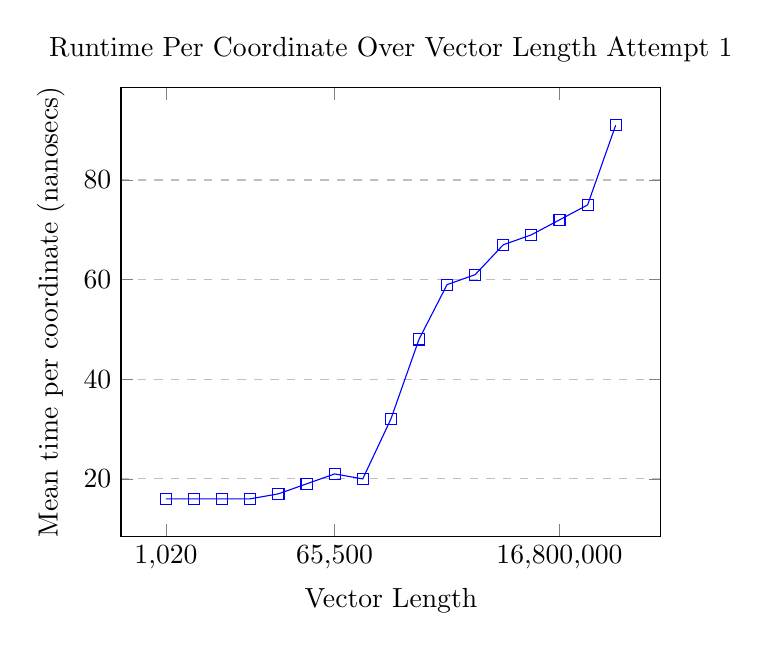
\begin{tikzpicture}
\begin{axis}[
    title={Runtime Per Coordinate Over Vector Length Attempt 1},
    xlabel={Vector Length},
    ylabel={Mean time per coordinate (nanosecs)},
    %xmin=0, xmax=100,
    %ymin=0, ymax=120,
    xtick={1024, 65536, 16777216},
    %ytick={0,20,40,60,80,100,120},
    ymajorgrids=true,
    grid style=dashed,
    xmode=log,
    log ticks with fixed point,
   % x filter/.code=\pgfmathparse{#1 + 6.90775527898214},
]
 
\addplot[
    color=blue,
    mark=square,
    ]
    coordinates {
    (1024, 16)
    (2048, 16)
    (4096, 16)
    (8192, 16)
    (16384, 17)
    (32768, 19)
    (65536, 21)
    (131072, 20)
    (262144, 32)
    (524288, 48)
    (1048576, 59)
    (2097152, 61)
    (4194304, 67)
    (8388608, 69)
    (16777216, 72)
    (33554432, 75)
    (67108864, 91)
    };
    
\end{axis}
\end{tikzpicture}

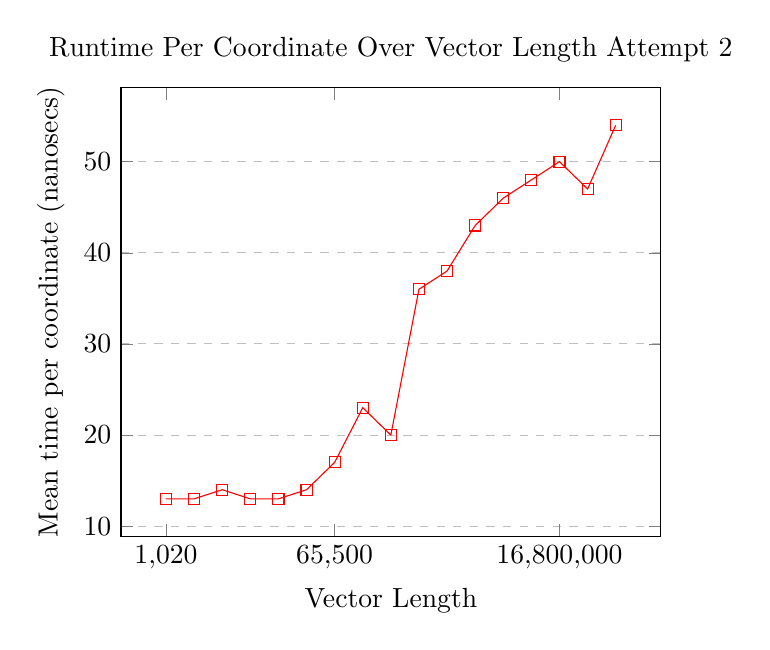
\begin{tikzpicture}
\begin{axis}[
    title={Runtime Per Coordinate Over Vector Length Attempt 2},
    xlabel={Vector Length},
    ylabel={Mean time per coordinate (nanosecs)},
    %xmin=0, xmax=100,
    %ymin=0, ymax=120,
    xtick={1024, 65536, 16777216},
    %ytick={0,20,40,60,80,100,120},
    ymajorgrids=true,
    grid style=dashed,
    xmode=log,
    log ticks with fixed point,
   % x filter/.code=\pgfmathparse{#1 + 6.90775527898214},
]
 
\addplot[
    color=red,
    mark=square,
    ]
    coordinates {
    (1024, 13)
    (2048, 13)
    (4096, 14)
    (8192, 13)
    (16384, 13)
    (32768, 14)
    (65536, 17)
    (131072, 23)
    (262144, 20)
    (524288, 36)
    (1048576, 38)
    (2097152, 43)
    (4194304, 46)
    (8388608, 48)
    (16777216, 50)
    (33554432, 47)
    (67108864, 54)
    };
    
\end{axis}
\end{tikzpicture}

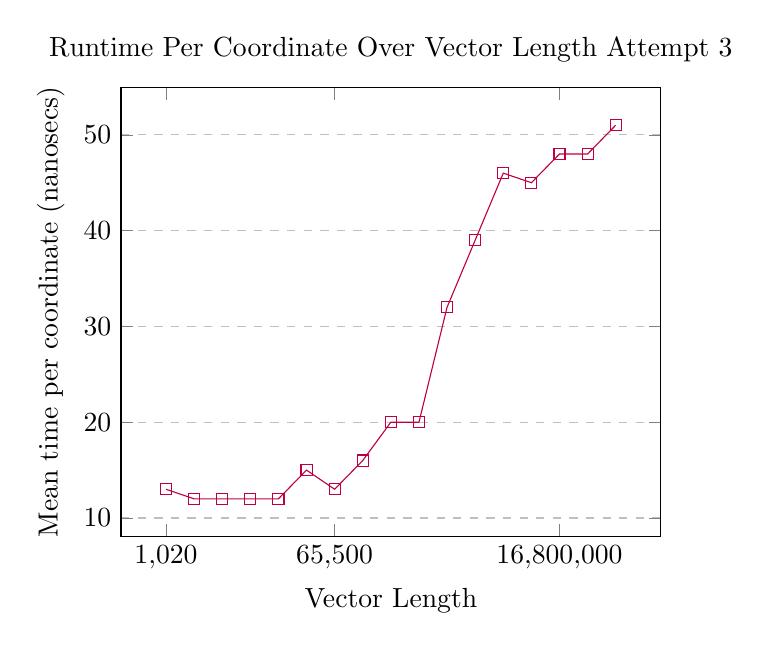
\begin{tikzpicture}
\begin{axis}[
    title={Runtime Per Coordinate Over Vector Length Attempt 3},
    xlabel={Vector Length},
    ylabel={Mean time per coordinate (nanosecs)},
    %xmin=0, xmax=100,
    %ymin=0, ymax=120,
    xtick={1024, 65536, 16777216},
    %ytick={0,20,40,60,80,100,120},
    ymajorgrids=true,
    grid style=dashed,
    xmode=log,
    log ticks with fixed point,
   % x filter/.code=\pgfmathparse{#1 + 6.90775527898214},
]
\addplot[
    color=purple,
    mark=square,
    ]
    coordinates {
    (1024, 13)
    (2048, 12)
    (4096, 12)
    (8192, 12)
    (16384, 12)
    (32768, 15)
    (65536, 13)
    (131072, 16)
    (262144, 20)
    (524288, 20)
    (1048576, 32)
    (2097152, 39)
    (4194304, 46)
    (8388608, 45)
    (16777216, 48)
    (33554432, 48)
    (67108864, 51)
    };
    
\end{axis}
\end{tikzpicture}



\end{document}








